\documentclass[a4paper,12pt]{article}
\usepackage{color}
\usepackage{graphicx, gensymb}
\usepackage{amsfonts, cancel, amssymb}
\usepackage{amsmath, amsthm, array, esvect, esint}
\usepackage{typearea, tikz, pgffor}
\usetikzlibrary{calc, quotes}
\usepackage[a4paper,left=2cm,right=2cm,top=2cm,bottom=3cm,bindingoffset=5mm]{geometry}
\newcommand\numberthis{\addtocounter{equation}{1}\tag{\theequation}}
\newcommand{\bra}{}
\newcommand{\kom}{}
\newcommand{\brak}{}
\newcommand{\braket}{}
\newcommand{\intx}{}
\newcommand{\intr}{}
\newcommand{\kla}{}
\newcommand{\klam}{}
\newcommand{\klammer}{}
\newcommand{\oper}{}
\newcommand{\tecxt}{}
\newcommand{\Bra}{}
\newcommand{\Ket}{}

\begin{document}

\title{03 Bindungstypen}
\author{Joachim Schwardt}
\date{\today}
\maketitle

%\section*{Aufgabe 1: Bindungstypen}
\section*{Aufgabe 2: Ionenkristall aus identischen Atomen}
\begin{figure}[h!]
\centering
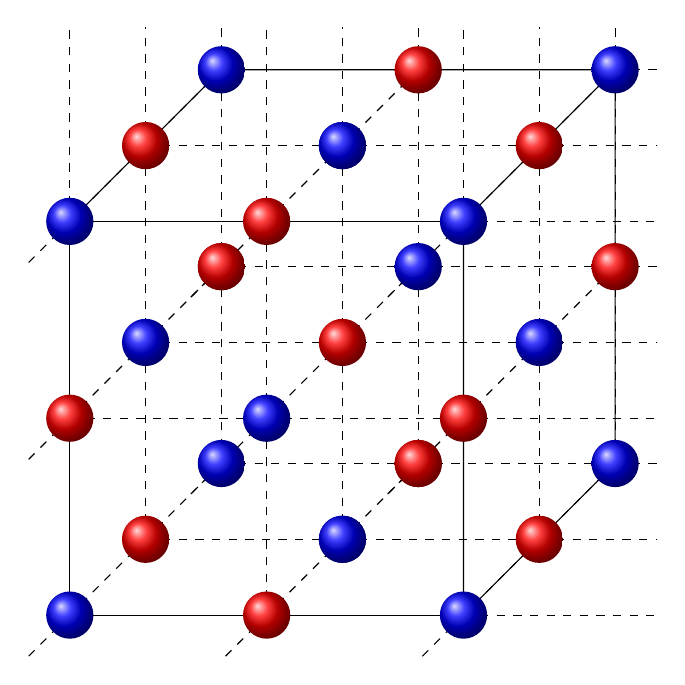
\begin{tikzpicture}[scale=2.5]
\clip (-2.6,-2.6,-2.6) rectangle (2.6,2.6,2.6);
%\foreach \r in {1, 1.414}{
  %\shade[ball color = gray, opacity=0.2] (0,0,0) circle (\r);}
\foreach \x in {-1,0,1}{
  \foreach \y in {-1,0,1}{
    \foreach \z in {-1,0,1}{
      \draw[dashed] (\x,\y,\z) -- (\x+1,\y,\z);
      \draw[dashed] (\x,\y,\z) -- (\x,\y+1,\z);
      \draw[dashed] (\x,\y,\z) -- (\x,\y,\z+1);}}}
\draw (-1,-1,1) --++ (2,0,0) --++ (0,2,0) --++ (-2,0,0) --++ (0,-2,0);
\draw (1,1,1) --++ (0,0,-2) --++ (0,-2,0) --++ (0,0,2) --++ (0,2,0);
\draw (-1,1,1) --++ (0,0,-2) --++ (2,0,0);
\foreach \x/\y/\z in {-1/-1/-1, -1/1/-1, 1/1/-1, 1/-1/-1, -1/0/0, 1/0/0, 0/-1/0, 0/1/0, -1/-1/1, -1/1/1, 1/1/1, 1/-1/1, 0/-1/0, 0/1/0, 0/0/-1, 0/0/1}{
  \shade[ball color = blue] (\x,\y,\z) circle (0.12);}
\foreach \x/\y/\z in {0/-1/-1, -1/0/-1, 0/1/-1, 0/0/0, 1/0/-1, 1/0/1, -1/0/1, -1/0/-1, 0/-1/-1, 0/-1/1, -1/1/0, 1/1/0, -1/-1/0, 1/-1/0, 0/1/1}{
  \shade[ball color = red] (\x,\y,\z) circle (0.12);}
\end{tikzpicture}
\end{figure}
Die Potentielle Energie eines Atoms ergibt sich als Summe über die Coulomb-Energie zu allen anderen Atomen im Gitter. Dafür benötigt man die Madelung-Konstante $\alpha$: %https://www.quora.com/What-is-the-number-of-integral-solutions-of-x-+-y-+-z-10
\begin{align*}
E_\tecxt\text{Mad,Na}&=\frac{e^2}{4\pi\epsilon_0R}\sum_{(x,y,z)\in\mathbb{Z}^3\setminus\{0\}}\frac{(-1)^{x+y+z}}{\sqrt{x^2+y^2+z^2}}=:\alpha\frac{e^2}{4\pi\epsilon_0R}=-6.76\,\tecxt\text{eV}\\
E_\tecxt\text{Mad,NaCl}&=\alpha\frac{e^2}{4\pi\epsilon_0R_\tecxt\text{NaCl}}=-4.46\,\tecxt\text{eV}
\end{align*}
Damit folgt für die Bindungsenergien:
\begin{align*}
E_\tecxt\text{B,Na}&=I_\tecxt\text{Na}+A_\tecxt\text{Na}+E_\tecxt\text{Mad,Na}=-2.40\,\tecxt\text{eV}\\
E_\tecxt\text{B,NaCl}&=I_\tecxt\text{Na}+A_\tecxt\text{Cl}+E_\tecxt\text{Mad,NaCl}=-2.93\,\tecxt\text{eV}
\end{align*}
NaCl ist also stabiler. \newpage
\section*{Aufgabe 3: Eindimensionaler Ionenkristall}
Sei bei $x=0$ ein positiv geladenes Ion. Der Abstand zum $j$-ten Ion ist dann $x_j=j\cdot R$ und das Vorzeichen der Ladung dieses Ions ist $z_j=(-1)^j$. Dann gilt:
\begin{align*}
\alpha&=\sum_{|j|\ge 1}\frac{z_j}{x_j/R}=2\sum_{j\ge 1}\frac{(-1)^j}{j}=-2\log 2
\end{align*}
Die Summe kann mit folgender Taylorreihe bestimmt werden:
\begin{align*}
\log(1+x)&=\int\frac{1}{1+x}\,\mathrm{d}x=\sum_{k\ge 0}(-1)^k\int x^k\,\mathrm{d}x=-\sum_{k\ge 1}\frac{(-1)^kx^k}{k}
\end{align*}
Sei $B=\frac{q^2}{4\pi\epsilon_0}$ und $U(r)=\frac{N}{2}(\alpha B/r+A/r^n)$. Dann findet man den Gleichgewichtsabstand $r_0$ durch die Bedingung $U'(r)=0$:
\begin{align*}
0&=U'(r_0)\propto\alpha\frac{B}{r_0^2}+n\frac{A}{r_0^{n+1}}\ \ \Rightarrow\ \ -\frac{nA}{\alpha B}=r_0^{n-1}
\end{align*}
Damit folgt für das Potential bei $r_0$:
\begin{align*}
U(r_0)&=\frac{\alpha BN}{2r_0}\kla\left( {1+\frac{A}{\alpha B}\frac{1}{r_0^{n-1}}} \right)=-\log 2\frac{Nq^2}{4\pi\epsilon_0r_0}\kla\left( {1-\frac{1}{n}} \right)
\end{align*}
%\section*{Aufgabe 4: Kovalente Bindung}

\end{document}